\documentclass[11pt]{article}
\usepackage[a4paper,margin=2.3cm]{geometry}
\usepackage{amsmath,amssymb,bm,mathtools}
\usepackage{booktabs,array}
\usepackage{enumitem}
\usepackage[dvipsnames]{xcolor}
\usepackage[most]{tcolorbox}
\usepackage{tikz}
\usetikzlibrary{decorations.pathreplacing}
\usepackage{microtype}
\usepackage[colorlinks=true,linkcolor=NavyBlue,citecolor=ForestGreen,urlcolor=NavyBlue]{hyperref}

\newtcolorbox{keybox}[1][]{colback=Gray!6,colframe=Gray!55,boxrule=0.5pt,arc=2pt,left=6pt,right=6pt,top=5pt,bottom=5pt,#1}
\newtcolorbox{warnbox}[1][]{colback=BrickRed!5,colframe=BrickRed!60,boxrule=0.6pt,arc=2pt,left=6pt,right=6pt,top=5pt,bottom=5pt,#1}
\newtcolorbox{ideabox}[1][]{colback=ForestGreen!5,colframe=ForestGreen!55,boxrule=0.6pt,arc=2pt,left=7pt,right=7pt,top=6pt,bottom=6pt,#1}

\newcommand{\herm}{^{\mathsf{H}}}
\newcommand{\T}{^{\mathsf{T}}}
\newcommand{\va}{\mathbf{a}}\newcommand{\vy}{\mathbf{y}}\newcommand{\vs}{\mathbf{s}}
\newcommand{\vn}{\mathbf{n}}\newcommand{\vz}{\mathbf{z}}\newcommand{\vp}{\mathbf{p}}
\newcommand{\mA}{\mathbf{A}}\newcommand{\mR}{\mathbf{R}}\newcommand{\mI}{\mathbf{I}}
\newcommand{\E}{\mathbb{E}}\newcommand{\C}{\mathbb{C}}
\newcommand{\kr}{\odot}

\title{\textbf{Virtual Arrays, the Difference Co-Array and Vectorization}\\[3pt]
\large How physical and virtual sensors work, and how to use them\\ in near-field cell-free XL-MIMO}
\author{Literature review and framework note (simple English)}
\date{\today}

\begin{document}
\maketitle

\begin{keybox}
\textbf{What this note answers.}
(1) Where the virtual co-array idea came from and why people moved to it;
(2) what a ``sensor'' is, and what \emph{physical} and \emph{virtual} sensors mean;
(3) how the difference co-array and vectorization work, step by step, with the mathematics;
(4) what earlier papers did, including Pinto and de~Lamare's work;
(5) how it can help our CAPE-based cell-free system --- and, honestly, where it cannot help;
(6) four new array-structure ideas for the near field.
\end{keybox}

%====================================================================
\section{Where the idea came from, and why}

\textbf{The old limit.} With $N$ physical antennas in a uniform linear array (ULA), a receiver can
separate at most $N-1$ directions. The number of users or sources you can resolve is tied to the
number of antennas, and each antenna costs money, space and one RF chain
\cite{vantrees2002oap}.

\textbf{First attempt (1968).} Minimum-redundancy arrays placed antennas at unequal spacings so that
the set of \emph{differences} between antenna positions contained as many distinct values as possible
\cite{moffet1968mra}. The idea was already there: what matters is not only where the antennas are,
but which \emph{distances} between pairs exist.

\textbf{The breakthrough: use second-order statistics.} If instead of the raw received signal we use
its \emph{covariance matrix}, the entries of that matrix depend on \emph{differences} of antenna
positions. Those differences form a much larger set than the antennas themselves, called the
\textbf{difference co-array}. Processing in this domain allows a receiver to identify
$\mathcal{O}(N^{2})$ sources with only $N$ physical antennas
\cite{pal2010nested,vaidyanathan2011coprime}.

\textbf{Closed-form designs.} Nested arrays \cite{pal2010nested} gave the first simple construction
whose difference co-array is a \emph{hole-free} (contiguous) virtual ULA, with a closed-form optimum.
Co-prime arrays \cite{vaidyanathan2011coprime} followed, with a co-array that has gaps (holes).

\begin{keybox}
\textbf{The motivation in one line.} Physical antennas are expensive; \emph{differences} between them
are free. By working in the covariance (second-order) domain we obtain a much larger ``virtual''
array, and therefore many more degrees of freedom and finer resolution, without adding hardware
\cite{pal2010nested,vaidyanathan2011coprime}.
\end{keybox}

\textbf{What was missing in a plain nested array.} A nested array by itself is still only $N$
physical antennas: if you process the received signal \emph{directly} (first-order), you get only
$N$ degrees of freedom and you also suffer side lobes from the sparse spacing. The extra
$\mathcal{O}(N^{2})$ degrees of freedom appear \emph{only} after you move to the covariance domain
and build the co-array \cite{pal2010nested}. This is exactly why people went from ``nested array''
to ``nested array \emph{plus} difference co-array plus vectorization''.

%====================================================================
\section{What is a ``sensor''? Physical vs.\ virtual}

In this literature \textbf{sensor $=$ antenna element}. A sensor is one receiving element with its
own RF chain. So ``$N$ sensors'' means ``$N$ antennas''.

\begin{center}
\renewcommand{\arraystretch}{1.25}
\begin{tabular}{@{}p{3.3cm}p{5.6cm}p{5.6cm}@{}}
\toprule
 & \textbf{Physical sensor (antenna)} & \textbf{Virtual sensor}\\
\midrule
What is it? & Real hardware on the panel & A \emph{position} that appears as a difference of two
 physical positions\\
Does it exist? & Yes, you can touch it & No. It exists only inside the covariance matrix\\
Costs an RF chain? & Yes & No\\
Receives energy? & Yes & \textbf{No} --- it carries no extra signal power\\
What does it give? & Signal + array gain & Extra \emph{degrees of freedom} and \emph{resolution}\\
\bottomrule
\end{tabular}
\end{center}

\begin{warnbox}
\textbf{Very important, and often misunderstood.} A virtual sensor does \emph{not} collect any new
signal energy. It increases the number of \emph{parameters} (directions, ranges, users) that can be
identified and sharpens resolution, but it gives \emph{no} extra beamforming gain and \emph{no} extra
received SNR \cite{pal2010nested,liu2015remarks}. Any claim of a ``$N^{2}$-antenna array for free''
must be read as ``$N^{2}$ \emph{identifiable parameters}'', not ``$N^{2}$ antennas''.
\end{warnbox}

%====================================================================
\section{How the difference co-array and vectorization work (step by step)}

\subsection{Step 1 --- the physical received signal}
Let the array have $N$ antennas at positions $x_{1},\dots,x_{N}$ (in units of $d=\lambda/2$), and let
$K$ sources (users) arrive from angles $\theta_{1},\dots,\theta_{K}$. The received snapshot at time
$t$ is
\begin{equation}
\vy(t)=\mA\,\vs(t)+\vn(t),\qquad \vy(t)\in\C^{N\times1},
\label{eq:phys}
\end{equation}
\textit{Here $\vy(t)$ is the vector of what the $N$ antennas measure at time $t$ (one complex number
per antenna), so its size is $N\times1$. $\mA=[\va(\theta_{1}),\dots,\va(\theta_{K})]$ is the
steering matrix: each column $\va(\theta_{k})$ says how source $k$ appears across the antennas.
$\vs(t)$ holds the $K$ source symbols at time $t$, and $\vn(t)$ is the receiver noise, assumed white
with power $\sigma^{2}$.} The steering vector entries are
\begin{equation}
[\va(\theta)]_{n}=e^{\,\jmath\frac{2\pi}{\lambda}x_{n}\sin\theta},\qquad n=1,\dots,N .
\label{eq:steer}
\end{equation}
\textit{Here $[\va(\theta)]_{n}$ is the phase that a plane wave from angle $\theta$ produces at
antenna $n$; $x_{n}$ is that antenna's position and $\lambda$ the wavelength. Note this is the
\emph{far-field} (flat wavefront) model --- we return to this point in Section~6.}

\subsection{Step 2 --- the covariance matrix exposes the differences}
Assume the sources are uncorrelated with powers $p_{1},\dots,p_{K}$. The covariance is
\begin{equation}
\mR=\E\big[\vy(t)\vy(t)\herm\big]=\mA\,\mathrm{diag}(\vp)\,\mA\herm+\sigma^{2}\mI_{N},
\label{eq:cov}
\end{equation}
\textit{Here $\mR$ is the $N\times N$ covariance matrix (how each antenna's signal correlates with
every other antenna's). $\vp=[p_{1},\dots,p_{K}]\T$ collects the source powers,
$\mathrm{diag}(\vp)$ puts them on a diagonal, $\sigma^{2}$ is the noise power, and $\mI_{N}$ is the
identity matrix.} Looking at one entry of $\mR$ makes the key point visible:
\begin{equation}
[\mR]_{m,n}=\sum_{k=1}^{K}p_{k}\,e^{\,\jmath\frac{2\pi}{\lambda}(x_{m}-x_{n})\sin\theta_{k}}
+\sigma^{2}\delta_{m,n}.
\label{eq:entry}
\end{equation}
\textit{Here $[\mR]_{m,n}$ is the correlation between antenna $m$ and antenna $n$, and
$\delta_{m,n}=1$ if $m=n$ and $0$ otherwise. The phase depends only on the \textbf{difference}
$x_{m}-x_{n}$.} This is the whole trick: the covariance behaves as if there were an antenna at every
difference position. The set of these positions is the \textbf{difference co-array}
\begin{equation}
\mathbb{D}=\{\,x_{m}-x_{n}\ :\ 1\le m,n\le N\,\}.
\label{eq:coarray}
\end{equation}
\textit{Here $\mathbb{D}$ is the list of all differences between pairs of physical antenna positions.
Each element of $\mathbb{D}$ is one \emph{virtual sensor}.}

\subsection{Step 3 --- vectorization turns the co-array into a ``received vector''}
Stack the columns of $\mR$ into one long vector. Using the identity
$\mathrm{vec}(\mA\,\mathrm{diag}(\vp)\,\mA\herm)=(\mA^{*}\kr\mA)\vp$,
\begin{equation}
\boxed{\;\vz=\mathrm{vec}(\mR)=\big(\mA^{*}\kr\mA\big)\vp+\sigma^{2}\mathrm{vec}(\mI_{N}),
\qquad \vz\in\C^{N^{2}\times1}.\;}
\label{eq:vec}
\end{equation}
\textit{Here $\vz$ is the vectorized covariance: a single long column of length $N^{2}$.
$\mathrm{vec}(\cdot)$ stacks matrix columns on top of each other, $(\cdot)^{*}$ is the complex
conjugate, and $\kr$ is the Khatri--Rao (column-wise Kronecker) product. $\vp$ is again the vector of
source powers.} The crucial structure is that column $k$ of $\mA^{*}\kr\mA$ is
$\va^{*}(\theta_{k})\otimes\va(\theta_{k})$, whose entries are
$e^{\jmath\frac{2\pi}{\lambda}(x_{m}-x_{n})\sin\theta_{k}}$ --- exactly the steering vector of a
\emph{virtual array} sitting at the difference positions \eqref{eq:coarray}
\cite{pal2010nested}. So \eqref{eq:vec} reads like ``received signal $=$ virtual steering matrix
$\times$ source powers $+$ a deterministic noise term''.

\begin{keybox}
\textbf{Size comparison (the professor's point).}
Regular or nested array: $\vy=\mA\vs+\vn$ with $\vy$ of size $N\times1$ --- $N$ physical sensors.\\
Difference co-array $+$ vectorization: $\vz=(\mA^{*}\kr\mA)\vp+\sigma^{2}\mathrm{vec}(\mI)$ with
$\vz$ of size $N^{2}\times1$ --- physical \emph{and} virtual sensors together.
\end{keybox}

\subsection{Step 4 --- remove duplicates and restore rank}
Many differences in \eqref{eq:coarray} repeat, so $\vz$ is reduced to the distinct lags, giving a
virtual array $\tilde{\vz}$ with $|\mathbb{D}|$ elements. Two difficulties then appear:
\begin{enumerate}[leftmargin=1.5em,itemsep=1pt]
\item \textbf{Holes.} For a co-prime array $\mathbb{D}$ has gaps, so the virtual array is not a
      contiguous ULA; the gaps must be filled by interpolation (for example nuclear-norm
      minimisation) or avoided by design \cite{liu2017interp}. \emph{Nested arrays avoid this: their
      difference co-array is hole-free} \cite{pal2010nested}.
\item \textbf{Rank-one problem.} In \eqref{eq:vec} the ``signal'' $\vp$ is deterministic, so
      $\tilde{\vz}$ behaves like a \emph{single snapshot} of fully coherent sources and subspace
      methods such as MUSIC fail \cite{liu2015remarks}.
\end{enumerate}
The classical fix is \textbf{spatial smoothing}: split the virtual ULA into overlapping subarrays and
average their covariances,
\begin{equation}
\mR_{\mathrm{ss}}=\frac{1}{L_{v}}\sum_{i=1}^{L_{v}}\tilde{\vz}_{i}\tilde{\vz}_{i}\herm ,
\label{eq:ss}
\end{equation}
\textit{Here $\tilde{\vz}_{i}$ is the portion of the virtual array vector taken by the $i$-th
subarray (a sliding window), $L_{v}$ is the number of such subarrays, and $\mR_{\mathrm{ss}}$ is the
smoothed covariance, which is full rank and can be given to MUSIC.} Liu and Vaidyanathan later showed
the smoothing step is not strictly necessary: the same noise subspace can be obtained directly from
an easier-to-compute matrix \cite{liu2015remarks}.

\subsection{The nested array geometry (the one used in this literature)}
A two-level nested array is the union of two ULAs: an inner one with $N_{1}$ antennas at spacing $d$,
and an outer one with $N_{2}$ antennas at spacing $(N_{1}+1)d$ \cite{pal2010nested}:
\begin{equation}
\mathbb{S}=\underbrace{\{\,m\,d\ :\ m=1,\dots,N_{1}\}}_{\text{inner, dense}}\ \cup\
\underbrace{\{\,n(N_{1}+1)d\ :\ n=1,\dots,N_{2}\}}_{\text{outer, sparse}} .
\label{eq:nested}
\end{equation}
\textit{Here $\mathbb{S}$ is the set of physical antenna positions, $N_{1}$ and $N_{2}$ are the
numbers of antennas in the inner and outer parts, and $d=\lambda/2$. The total is $N=N_{1}+N_{2}$
antennas.} Its difference co-array is a \emph{contiguous} virtual ULA running from
$-(N_{2}(N_{1}+1)-1)$ to $+(N_{2}(N_{1}+1)-1)$, i.e.
\begin{equation}
|\mathbb{D}|=2N_{2}(N_{1}+1)-1\ \approx\ \tfrac{N^{2}}{2}\quad\text{virtual sensors},
\label{eq:dof}
\end{equation}
\textit{Here $|\mathbb{D}|$ is how many virtual sensors the co-array contains. With
$N_{1}=N_{2}=N/2$ this is about $N^{2}/2$: from $N$ real antennas we obtain roughly $N^{2}/2$ virtual
ones.}

\begin{center}
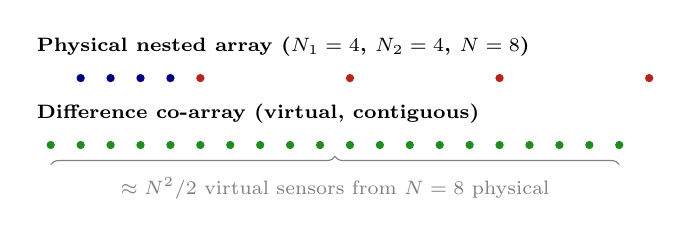
\begin{tikzpicture}[scale=1,dot/.style={circle,fill=#1,minimum size=3pt,inner sep=0pt}]
\node[font=\scriptsize\bfseries,anchor=west] at (-0.3,1.0) {Physical nested array ($N_1=4$, $N_2=4$, $N=8$)};
\foreach \x in {1,2,3,4} \node[dot=NavyBlue] at (\x*0.38,0.6) {};
\foreach \x in {5,10,15,20} \node[dot=BrickRed] at (\x*0.38,0.6) {};
\node[font=\scriptsize\bfseries,anchor=west] at (-0.3,0.15) {Difference co-array (virtual, contiguous)};
\foreach \x in {0,1,...,19} \node[dot=ForestGreen] at (\x*0.38,-0.25) {};
\draw[decorate,decoration={brace,amplitude=3pt},Gray] (0,-0.5) -- (19*0.38,-0.5)
 node[midway,below,font=\scriptsize,yshift=-1pt]{$\approx N^2/2$ virtual sensors from $N=8$ physical};
\end{tikzpicture}
\end{center}

%====================================================================
\section{What earlier papers did}

\begin{center}
\renewcommand{\arraystretch}{1.2}
\begin{tabular}{@{}p{4.3cm}p{10.3cm}@{}}
\toprule
\textbf{Work} & \textbf{Contribution}\\
\midrule
Moffet \cite{moffet1968mra} & Minimum-redundancy arrays: maximise the distinct differences; no
closed form.\\
Pal \& Vaidyanathan \cite{pal2010nested} & \textbf{Nested arrays}: closed-form two-level design whose
difference co-array is a hole-free virtual ULA; $\mathcal{O}(N^{2})$ degrees of freedom from $N$
sensors using second-order statistics.\\
Vaidyanathan \& Pal \cite{vaidyanathan2011coprime} & \textbf{Co-prime arrays}: two co-prime ULAs;
co-array has holes but the design is flexible.\\
Liu \& Vaidyanathan \cite{liu2015remarks} & Analysed the spatial-smoothing step in co-array MUSIC and
showed an equivalent, cheaper construction (no smoothing needed).\\
Liu \emph{et al.} \cite{liu2017interp} & Co-array \emph{interpolation} (nuclear-norm minimisation) to
fill the holes of co-prime co-arrays.\\
Liu \& Vaidyanathan \cite{liu2016supernested} & \textbf{Super nested arrays}: keep the hole-free
co-array but reduce \emph{mutual coupling} between close antennas.\\
Sum/difference designs \cite{zhou2020revshift,shi2025noncirc} & Use both \emph{sum} and
\emph{difference} lags (e.g.\ for non-circular signals) for still more degrees of freedom.\\
Near-field variants \cite{wang2016csna,zhang2019symdouble,chen2023hybrid} & \textbf{Symmetric} nested
arrays (SNA, compressed SNA, symmetric double-nested) for near-field and mixed near/far-field
localisation --- see Section~6.\\
\textbf{Pinto \& de~Lamare} \cite{pinto2023sra} & \textbf{Co-array for communications} (not only
DOA): uplink multiuser MIMO with nested/co-prime arrays; MMSE and SIC receivers on the difference
co-array; sum-rate analysis.\\
\bottomrule
\end{tabular}
\end{center}

\subsection{Pinto and de~Lamare's work in detail}
The paper is \emph{``Study of Multiuser Multiple-Antenna Wireless Communications Systems Based on
Super-Resolution Arrays''} by S.~F.~B.~Pinto and R.~C.~de~Lamare \cite{pinto2023sra} (arXiv:2312.06033,
December 2023; a related version appeared at EUSIPCO~2023, Helsinki, in the \emph{MIMO and Array
Processing} session). From its abstract and section outline:
\begin{itemize}[leftmargin=1.4em,itemsep=1pt]
\item \textbf{Setting:} the \emph{uplink} of a multiuser system where users transmit to a
      multiple-antenna base station equipped with \emph{super-resolution} (sparse) arrays.
\item \textbf{Arrays:} \emph{co-prime} and \emph{two-level nested} arrays, handled by one common
      procedure.
\item \textbf{Receivers:} linear MMSE receive filters, plus linear and \emph{successive interference
      cancellation} (SIC) receivers, designed to process the signals \emph{of the difference
      co-array}.
\item \textbf{Analysis:} closed-form expressions for the achievable sum-rates.
\item \textbf{Claims:} the proposed systems outperform standard-array systems that use \emph{more}
      antenna elements, with gains in achievable rate and bit-error rate and savings in antennas and
      energy.
\end{itemize}

\begin{warnbox}
\textbf{Honest limitation of this review.} The network in this environment blocks direct downloads
from arXiv and the publisher sites, so I could read only the abstract, section outline and indexed
summaries of \cite{pinto2023sra} --- \textbf{not} the full derivations or the numerical results.
The description above is therefore faithful to the abstract but the exact receiver derivation and
simulation parameters must be checked against the paper itself before you reproduce or cite them.
\end{warnbox}

\textbf{Which technique to adopt for comparison.} For our purpose the right baseline is exactly
\cite{pinto2023sra}: a \textbf{two-level nested array \eqref{eq:nested} with the difference co-array
and vectorization \eqref{eq:vec}}, because (i) it is the version designed for \emph{communications}
(MMSE/SIC receivers, sum-rate, BER) rather than pure DOA, (ii) it comes from the same group as our
work, and (iii) the nested geometry gives a hole-free co-array, so no interpolation step is needed.

%====================================================================
\section{How this can help our work --- and where it cannot}

Our pipeline is: pilots $\rightarrow$ per-AP angle/range estimate $\rightarrow$ CAPE cross-AP position
fusion $\rightarrow$ channel reconstruction $\rightarrow$ cross-AP list SIC detection. The co-array
belongs in the \emph{first} step.

\begin{center}
\renewcommand{\arraystretch}{1.2}
\begin{tabular}{@{}p{5.1cm}p{9.5cm}@{}}
\toprule
\textbf{Where it helps} & \textbf{Why}\\
\midrule
Sharper per-AP parameter estimates & The virtual aperture is much larger than the physical one, and
resolution improves with aperture, so the angle/range candidates fed to CAPE are far more accurate
\cite{pal2010nested}.\\
More identifiable users & Up to $\mathcal{O}(N^{2})$ sources instead of $N$ --- useful when the
number of users per AP is large \cite{pal2010nested,vaidyanathan2011coprime}.\\
Fewer RF chains & The same resolution with fewer physical antennas, i.e.\ lower hardware cost
\cite{pinto2023sra}.\\
Side-lobe robustness & The co-array processing works on lags, which is a different and often more
robust way of handling the ambiguity that worries us with sparse arrays \cite{liu2015remarks}.\\
\bottomrule
\end{tabular}
\end{center}

\begin{warnbox}
\textbf{Four honest limitations you must plan for.}
\begin{enumerate}[leftmargin=1.5em,itemsep=1pt]
\item \textbf{No extra energy.} Virtual sensors add degrees of freedom and resolution, \emph{not}
      received power. They cannot improve the beamforming gain of the data detector by themselves
      \cite{pal2010nested}.
\item \textbf{Needs many snapshots.} The covariance $\mR$ in \eqref{eq:cov} must be \emph{estimated}
      from data. Our pilot phase gives only $\tau=K$ snapshots, which is very few, so
      $\hat{\mR}$ is noisy and the co-array gain shrinks \cite{liu2015remarks}.
\item \textbf{Degrees of freedom are not our bottleneck.} In our setting $K=8$ users and $N=63$
      antennas per AP, so $K\ll N$: we do \emph{not} need $\mathcal{O}(N^{2})$ degrees of freedom.
      The benefit for us would be \emph{resolution}, not source count.
\item \textbf{The near field breaks the standard co-array} --- see Section~6. This is the most
      serious issue for our system.
\end{enumerate}
\end{warnbox}

%====================================================================
\section{The near-field catch (critical)}

Equation \eqref{eq:steer} assumed a \emph{flat} wavefront. In the near field the wavefront is curved,
so the phase contains an extra range-dependent (quadratic) term and the amplitude also varies across
the array. Consequently the neat cancellation that produced a clean virtual ULA in \eqref{eq:entry}
no longer holds: the ULA behaviour of the difference co-array \emph{breaks down} for near-field
sources because of curved wavefronts and range-dependent attenuation
\cite{wang2016csna,zhang2019symdouble}.

\textbf{The known remedy: symmetry.} If the array is made \emph{symmetric} about its centre, the
quadratic range term cancels in particular lag combinations, which restores a usable co-array and
even allows the range to be recovered. This is why the near-field literature uses \emph{symmetric}
nested arrays (SNA), compressed symmetric nested arrays (CSNA), symmetric double-nested and symmetric
extended nested arrays \cite{wang2016csna,zhang2019symdouble,chen2023hybrid}. A typical procedure is:
estimate the angles by spatial-smoothing MUSIC on the difference co-array, then obtain each range by
a one-dimensional peak search using the estimated angle \cite{zhang2019symdouble}.

\begin{keybox}
\textbf{So, for our hybrid near/far-field system:} a plain two-level nested array with the standard
difference co-array is \emph{not} directly valid on the near-field links. Either restrict the
co-array processing to the far-field links, or adopt a \emph{symmetric} structure. Our current ECA is
already symmetric about its centre, which is a useful starting point.
\end{keybox}

%====================================================================
\section{Four new structure ideas for the near field}

These are proposals, not results. Idea~1 is closest to existing work; Ideas~2--4 are, to my
knowledge, not published for near-field cell-free systems --- verify before claiming novelty.

\begin{ideabox}
\textbf{Idea 1 --- Symmetric nested co-array per AP (safest).}
Replace the ECA with a \emph{symmetric} two-level nested array so the difference co-array stays valid
in the near field \cite{wang2016csna,zhang2019symdouble}. \emph{Benefit:} hole-free co-array
\emph{and} near-field validity. \emph{Risk:} symmetric nested arrays already exist, so the novelty is
only in the cell-free application.
\end{ideabox}

\begin{ideabox}
\textbf{Idea 2 --- Cross-AP (distributed) co-array.}
Form the difference co-array \emph{across APs}, using the union of all AP antenna positions, instead
of inside one AP. Since CAPE already fuses several APs, the lag set becomes enormous and its
``virtual aperture'' spans the whole deployment. \emph{Benefit:} resolution limited by the
\emph{network} size, not the panel size; it matches CAPE naturally. \emph{Risk:} APs are not
phase-synchronous, so only non-coherent (power-domain) lags may be usable --- this must be checked
first.
\end{ideabox}

\begin{ideabox}
\textbf{Idea 3 --- Joint sum-and-difference co-array for the near field.}
Near-field phase contains both a linear (angle) and a quadratic (range) term, which naturally produce
\emph{sum} lags $x_{m}+x_{n}$ as well as difference lags. Designing the geometry so that
\emph{both} co-arrays are hole-free would give joint angle--range degrees of freedom in one step.
Sum-difference designs exist for far-field and non-circular signals
\cite{zhou2020revshift,shi2025noncirc}; extending them to near-field cell-free appears open.
\end{ideabox}

\begin{ideabox}
\textbf{Idea 4 --- Hybrid-field reconfigurable co-array.}
Our network is hybrid: some links are near-field, some far-field. Use the \emph{full} difference
co-array on far-field links (where it is exactly valid) and a \emph{symmetric sub-array} with
range-aware processing on near-field links, switching per link using the Rayleigh-distance test we
already compute. \emph{Benefit:} each link uses the processing that is actually valid for it.
\end{ideabox}

\begin{keybox}
\textbf{For the code comparison you asked for}, we use \emph{no} new idea: we implement the published
technique of \cite{pinto2023sra} --- a two-level nested array \eqref{eq:nested} with the difference
co-array and vectorization \eqref{eq:vec} --- and compare it against our ECA-based CAPE system on
BER, sum-rate, estimation error and localisation.
\end{keybox}

%====================================================================
\begin{thebibliography}{99}\small
\bibitem{vantrees2002oap} H.~L.~Van~Trees, \emph{Optimum Array Processing: Part IV of Detection,
Estimation, and Modulation Theory}. New York: Wiley, 2002.
\bibitem{moffet1968mra} A.~T.~Moffet, ``Minimum-redundancy linear arrays,'' \emph{IEEE Trans.
Antennas Propag.}, vol.~16, no.~2, pp.~172--175, 1968.
\bibitem{pal2010nested} P.~Pal and P.~P.~Vaidyanathan, ``Nested arrays: A novel approach to array
processing with enhanced degrees of freedom,'' \emph{IEEE Trans. Signal Process.}, vol.~58, no.~8,
pp.~4167--4181, 2010.
\bibitem{vaidyanathan2011coprime} P.~P.~Vaidyanathan and P.~Pal, ``Sparse sensing with co-prime
samplers and arrays,'' \emph{IEEE Trans. Signal Process.}, vol.~59, no.~2, pp.~573--586, 2011.
\bibitem{liu2015remarks} C.-L.~Liu and P.~P.~Vaidyanathan, ``Remarks on the spatial smoothing step in
coarray MUSIC,'' \emph{IEEE Signal Process. Lett.}, vol.~22, no.~9, pp.~1438--1442, 2015.
\bibitem{liu2016supernested} C.-L.~Liu and P.~P.~Vaidyanathan, ``Super nested arrays: Linear sparse
arrays with reduced mutual coupling---Part I: Fundamentals,'' \emph{IEEE Trans. Signal Process.},
vol.~64, no.~15, pp.~3997--4012, 2016.
\bibitem{liu2017interp} C.-L.~Liu, P.~P.~Vaidyanathan, and P.~Pal, ``Coprime coarray interpolation
for DOA estimation via nuclear norm minimization,'' in \emph{Proc. IEEE ISCAS}, 2016, pp.~2639--2642.
\bibitem{zhou2020revshift} C.~Zhou \emph{et al.}, ``A reversed and shift sparse array scheme based on
the difference and sum co-array,'' arXiv:2011.13172, 2020.
\bibitem{shi2025noncirc} J.~Shi \emph{et al.}, ``A novel sparse sum and difference co-array with low
redundancy and enhanced DOF for non-circular signals,'' arXiv:2504.16675, 2025.
\bibitem{wang2016csna} W.~Wang \emph{et al.}, ``Compressed symmetric nested arrays and their
application for direction-of-arrival estimation of near-field sources,'' \emph{Sensors}, vol.~16,
no.~11, art.~1939, 2016.
\bibitem{zhang2019symdouble} X.~Zhang \emph{et al.}, ``Localization of mixed near-field and far-field
sources using symmetric double-nested arrays,'' \emph{IEEE Trans. Antennas Propag.}, 2019.
\bibitem{chen2023hybrid} Y.~Chen \emph{et al.}, ``Hybrid near- and far-field source localization using
symmetric sparse array,'' \emph{IEEE}, 2023, doc.~10069591.
\bibitem{pinto2023sra} S.~F.~B.~Pinto and R.~C.~de~Lamare, ``Study of multiuser multiple-antenna
wireless communications systems based on super-resolution arrays,'' arXiv:2312.06033, Dec.\ 2023
(related version: EUSIPCO~2023, Helsinki).
\bibitem{haider2026vtc} N.~Haider and R.~C.~de~Lamare, ``Cross-AP channel estimation and interference
cancellation for near-field cell-free XL-MIMO systems,'' submitted to IEEE VTC, 2026.
\end{thebibliography}

\end{document}
